\section{System Architecure}
\label{sec:systemarch}

% This was corrected in my version... (Joir-dan performing diff 2010-06-30)
This section presents ontology and corpora, query processing, ranking queries, and query executing.

\subsection{Using Ontology and Corpora} 
\label{sec:ontology_corpora}

Morpheus uses an ontology that contains categories of a particular realm of interest. Every leaf node in the ontology is associated with a corpus of words belonging to a category.  For example, we have constructed an automotive ontology containing categories relevant to the automotive realm. This ontology provides a structure for reference in the following sections.

%% Comment made by Joir-dan (2010-06-29)
 %%Need to remove any references to Markov Blanket... since we abandoned that ship a while ago... 

Morpheus uses the DBpedia categories, Wikipedia pages and the WordNet synset heterarchy to construct ontologies. This approach is motivated by YAGO \cite{Suchanek2009phd}. First a realm is mapped to a DBpedia category \cite{Bizer2009}. 
Then a \emph{Markov Blanket} \cite{PRIS} is created covering all neighboring categories and using the DBpedia ontology properties \emph{broader} and \emph{narrower}. From here, the system recursively includes all categories up to the root.  

%% ^^^ Needs to remove references to blanket

Once we have the categories belonging to a particular realm, we associate them with WordNet synsets using an approach similar to YAGO\cite{Suchanek2009phd}. We determine a \emph{head noun} in the category name and search for it in the WordNet synsets. DBpedia categories having no WordNet synset match are excluded from our ontology. 

To build a corpus for each of the leaf nodes in the ontology, 
we extract \emph{terms} from the Wikipedia pages associated with the 
the DBpedia categories. From this term corpus, 
we can find the likelihood of a term belonging to a particular category. This assists in categorizing terms in a \emph{path-follower} query.
The likelihood is determined by the probability of a category given a term 
using \textit{Bayes Rule} (Eq. \ref{eq:bayesrule}), since we can 
easily obtain the term-category and term-corpus probabilities as 
relative frequencies. 

%% Comment by Joir-dan 2010-06-30: Term should prolly be replaced by n-gram

\begin{equation}
\label{eq:bayesrule}
P (category | term) = \frac{P(term | category) P(category)}{P(term)}
\end{equation}    

In addition, we evaluate Latent Dirichlet Allocation (LDA) to identify latent topics of the documents in a corpus \cite{Blei2003latentdirichlet}.  LDA is Bayesian model represents a document in the corpus by distributions over topics, and a topic itself is a distribution over all  terms in the corpus.  For example, for the Wikipedia pages, the latent topics reflect the thematic structure of the pages. Thus, LDA can discover relevant topic proportions in a document using posterior inference \cite{Blei2003latentdirichlet}. Additionally, given a text document, using LDA we could tag related documents by matching the similarity over the estimated topic proportions, which is useful in the ontology and corpora building.  Due to its fully generative semantics, even at the level of documents, LDA could address the drawbacks (such as dimensionality and failure in finding the discriminative set of words for a document) of frequency based approaches such as TF-IDF, LSI, and pLSI.


\subsection{ Recording}
\label{sec:query_processing}
  
%% Was edited and shortened by Joir-dan and Wilson (2010-06-29)
The \emph{Query Resolution Recorder} (QRR) is an instrumented web browser that records the interactions of a path-finder answering a question. The path-finder also uses the tool to identify ontological categories associated with search terms. Morpheus stores the query together with its terms and categories as an SSQ (Figure \ref{fig:ssq_example}). Using the QRR, the path-finder is also able to identify where answers can be found within traversed pages.

%% Was added by Joir-dan and Wilson (2010-06-29)... but may need to be better formatted
\begin{figure}[t]
\label{fig:ssq_example}
("An  1997 Toyota Camry V6 has what size tires", 
     (1997: Date, Toyota: Manufacturer, Camry: Model, V6: Engine ),
     (tire: Part, size: Measurement))
 
%% Comment made by Joir-dan Gumbs (2010-06-29) 
%%Need to talk a bit about this SSQ Structure: Does anyone see anything wrong with this representation?
\caption{An example SSQ for the question: A 1997 Toyota Camry V6 has what size tires?}
\end{figure} 

%% Edited by Joir-dan and Wilson (2010-06-29)
The \emph{Query Resolution Method} (QRM) is a data structure that models the
question answering process. A QRM represents a generalized executable realization of the search process that the path-finder followed. The QRM is able to reconstruct the page search path followed by the path-finder. Each QRM contains an \emph{ontological realm}, an SSQ, and information to support the query answering process. For each dynamic page, it stores the list of inputs to the URL such as form inputs and the possible reference outputs (highlighted portions of the web page).


% NLP arch. 
% This may need to be moved somewhere... but not sure where.... Joir-dan Gumbs (2010-06-29)

Queries inserted by path-followers take a different approach. The Morpheus search system parses, tags, and processes the queries in order to pull important n-grams. The system then assigns the most probable realm to the query using \textit{realm}|\textit{n-gram} priors calculated from realm-specific corpora. Once the realm is assigned, an ontology search is performed to assign classes to the n-grams. An SSQ is constructed and the system attempts to match this SSQ to a query path created by a path-finding user. Rather than matching n-grams, the goal is to match input and output classes, since the paths can potentially answer similar queries.


\subsection{Ranking} 
\label{sec:qrm_ranking}

To answer a user's query, a \textit{candidate
SSQ}, Morpheus finds similar SSQs that belong to QRMs in the Morpheus data store (a \textit{qualified SSQ}). We need a similarity measure to match the candidate SSQ
with a qualified SSQ. For the SSQ similarity, we
consider the SSQ components such as query-realm, input
terms and output terms, and their assigned categories or classes [To be changed]. The,
\textit{category divergence} of two categories characteristics their 
similarity based on an ontology class heterarchy. 
It is motivated by the concept of multiple
dispatch in CLOS and Dylan programming for generic function \emph{type} matches. 

We consider the category match as a type match and we use 
\emph{category divergence} to calculate the relevance between 
the candidate SSQ and a qualified SSQ. Each qualified SSQ will 
have input terms, output terms, and associated classes, and one realm (from QRM). 
For the candidate SSQ, the relevant categories for terms 
are determined from the NLP engine and corpora. The calculation of a realm 
for a candidate query is done using the n-grams found within said query 
and the probabilities (if any) found using frequencies within the database.
We match QRMs that belong to the same \emph{realm} of the candidate SSQ. 
The relevance of a qualified SSQ to the candidate SSQ is 
determined by aggregating the divergence measure of input-term-categories 
associated with them. In addition, we order QRMs in the data store 
by decreasing relevance. The order provides a ranking for the results 
to the user. The following subsection describes \emph{category divergence} 
in detail.

\subsubsection{Catgeory Divergence}
\label{sec:ctd}

We employ a quasimetric, \textit{category
divergence (cd)},
between a source category and a target category using the \textit{topological
structure} of the categories in an ontology. We write $S \prec T$ for the
reflexive
transitive closure of the supercategory relation. Let $d(P,Q)$ represent the hop
distance in the directed ontology inheritance graph from $P$ to $Q$. The
divergence between a source and target category ranges from zero (for identical
categories) to one (for type incompatible categories). Let $S$ be the source
category, $T$ be
the target category, and $C$ be a least common ancestor category of $S$ and
$T$ i.e., one that minimizes $d(S,C) + d(T,C)$. The category divergence between $S$ and $T$ is defined given by:

\begin{equation}
cd(S, T) = \begin{cases}
0 & S.{Uri} \equiv T.{Uri}\\
d(S, T)/(3h) & S \prec T\\
1 & T \prec S\\
(d(S,root) + d(S,C) \\ \ \ \ \ + d(T,C))/(3h) & otherwise
\end{cases}
\end{equation}

\noindent where $h$ is the height of the ontology tree.

Note, if $S \prec T$ and $S \not\prec Q$ then $cd(S,T) <
cd(S,Q)$, that is, the divergence of a source category to a target
ancestor category is smaller than the divergence of a source category to any
category that is not an ancestor. This is an important property in
determining the compatibility of categories for answering queries.  If a
SSQ answers queries concerning an ancestor category, it is more relevant
that a SSQ that answers queries from any non-ancestral category.

% Algorithm 1: figure  
\begin{figure}[t]
\centering
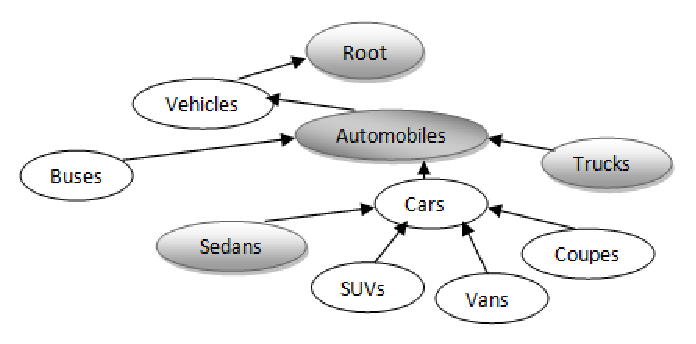
\includegraphics[width=85mm]{img/automotive_ontology.eps}
\caption{An abbreviated man-made automotive ontology - arrows represent inheritance relationships between the ontological classes.}
\label{fig:automotive_ontology}
\end{figure}

Suppose we want to find the category divergence between \textit{Sedans}
and \textit{Trucks} (Figure \ref{fig:automotive_ontology}). 
\textit{Sedans} is the subcategory of \textit{Cars}, and \textit{Trucks}
is the subcategory of \textit{Automobiles}. Therefore, the least common ancestor ($C$)
for these twoThis section presents ontology and copora, Query processing, ranking queries, and the query resolution mechanism. categories is \textit{Automobiles}. In addition, the tree height \textit{h = 4}.
So, the normalized divergence $cd$\textit{(Sedans, Trucks)} is \textit{7/12}
that is calculated from \textit{d(Sedans, Root) = 4}, \textit{d(Sedans, Automobiles) = 2}, and \textit{d(Trucks, Automobiles) = 1}.


\subsection{Executing} 

Once we have relevant QRMs through QRM ranking for a given user query, we can produce answers by re-running the pathways.

 The evaluation of this script by the QRE simulates the behavior of a human browsing the web, that is, clicking buttons to follow links, submitting forms, and highlighting of data to form a text answer.  The QRE assumes that becuase of the auto generated nature of deep web pages, the location of answers are the same irrespective of page changes.  It uses the relative XPath location to the answer node on HTML pages as described in \cite{Badica06}.


%When a user submits a new query to the Morpheus system, one or more stored QRMs are executed to obtain results. A QRM contains an XML script representing an algorithm that will obtain the required result. The evaluation of this script by the QRE simulates the behavior of a human browsing the web, that is, clicking buttons to follow links, submitting forms, highlighting data, cutting and pasting text, and constructing an answer in the form of a text string. There is greater complexity in dealing with web forms than with links. At present, the GET form submission method is used. This means that in preparation to submit a form, the Morpheus System builds a querystring consisting of name-value pairs. For a given form, there may be text fields, drop-down boxes, and among other components. In order to support form submission in such circumstances, the QRE performs different actions based upon the input type. For text fields, simply adding a key/value pair to the query string suffices. For a drop-down box, the QRE extracts the form element to find the appropriate value to include in the query string. It does this by examine each option in the drop-down and matching the user’s input to the text field in the option. The value attribute of the option is then added to the querystring. The value and text attributes of a dropdown option might be the same, but they are not guaranteed to be. All input data are kept in an internal table. The QRM script contains keys that allow the QRE to map SSQ inputs from the table to the appropriate form inputs. Furthermore, highlighted text segments collected during execution of the script are stored in the table. Once all actions in the script have been carried out, the QRE returns the textual answer this process has created. This answer is then be rendered in a browser displayed to the user.

